\subsection{UC20 - Visualizzazione richieste di spostamento pendenti}
\begin{figure}[H]
  \centering
  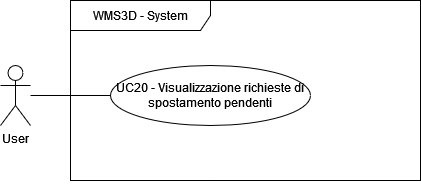
\includegraphics[width=0.8\textwidth]{UC_diagrams_11-20/UC20_sys.drawio.png}
   \caption{Diagramma UML UC20}
\end{figure}
\begin{figure}[H]
  \centering
  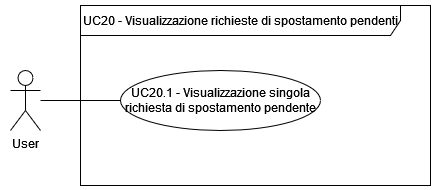
\includegraphics[width=0.8\textwidth]{UC_diagrams_11-20/UC20.drawio.png}
   \caption{Diagramma UML UC20 - dettaglio}
\end{figure}
\begin{itemize}
    \item \textbf{Attori:} User.
    \item \textbf{Pre-condizione:}  L'utente ha richiesto lo spostamento di un prodotto [UC19].
    \item \textbf{Post-condizione:} Si visualizzano tutte le richieste di spostamento inoltrate.
    \item \textbf{Scenario Principale:} L'utente dopo aver richiesto lo spostamento di un prodotto, può visualizzare per ogni richiesta i dettagli ad essa relativa [UC20.1].
    \item \textbf{Generalizzazioni:} -
    \item \textbf{Estensioni:} -
\end{itemize}


\subsubsection{UC20.1 - Visualizzazione singola richiesta di spostamento pendente}
\begin{figure}[H]
  \centering
  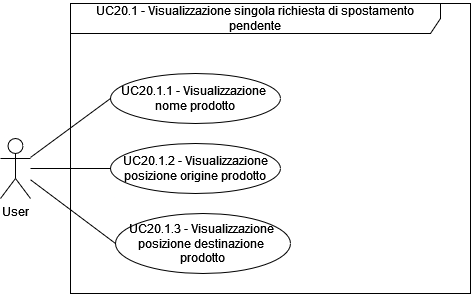
\includegraphics[width=0.8\textwidth]{UC_diagrams_11-20/UC20.1.drawio.png}
   \caption{Diagramma UML UC20.1}
\end{figure}
\begin{itemize}
    \item \textbf{Attori:} User.
    \item \textbf{Pre-condizione:}  L'utente ha richiesto lo spostamento di un prodotto [UC19] e vuole visualizzare lo stato della richiesta.
    \item \textbf{Post-condizione:} Si visualizza i dettagli della singola richiesta di spostamento.
    \item \textbf{Scenario Principale:} Per ogni singola richiesta di spostamento si visualizzano il nome [UC20.1.1], la posizione d'origine [UC20.1.2] e di destinazione [UC20.1.3] del prodotto oggetto della richiesta.
    \item \textbf{Generalizzazioni:} -
    \item \textbf{Estensioni:} -
\end{itemize}


\paragraph{UC20.1.1 - Visualizzazione nome prodotto}
\begin{itemize}
    \item \textbf{Attori:} User.
    \item \textbf{Pre-condizione:}  L'utente sta visualizzando una richiesta di spostamento.
    \item \textbf{Post-condizione:} L'utente visualizza il nome del prodotto.
    \item \textbf{Scenario Principale:} Per ogni singola richiesta di spostamento l'utente visualizza il nome del prodotto oggetto della richiesta.
    \item \textbf{Generalizzazioni:} -
    \item \textbf{Estensioni:} -
\end{itemize}


\paragraph{UC20.1.2 - Visualizzazione posizione origine prodotto}
\begin{itemize}
    \item \textbf{Attori:} User.
    \item \textbf{Pre-condizione:}  L'utente sta visualizzando una richiesta di spostamento.
    \item \textbf{Post-condizione:} L'utente visualizza la posizione originale del prodotto.
    \item \textbf{Scenario Principale:} Per ogni singola richiesta di spostamento l'utente visualizza la posizione originale del prodotto oggetto della richiesta.
    \item \textbf{Generalizzazioni:} -
    \item \textbf{Estensioni:} -
\end{itemize}


\paragraph{UC20.1.3 - Visualizzazione posizione destinazione prodotto}
\begin{itemize}
    \item \textbf{Attori:} User.
    \item \textbf{Pre-condizione:}  L'utente sta visualizzando una richiesta di spostamento.
    \item \textbf{Post-condizione:} L'utente visualizza la posizione di destinazione del prodotto.
    \item \textbf{Scenario Principale:} Per ogni singola richiesta di spostamento l'utente visualizza la posizione di destinazione del prodotto oggetto della richiesta.
    \item \textbf{Generalizzazioni:} -
    \item \textbf{Estensioni:} -
\end{itemize}